\documentclass{article}
\usepackage[a4paper, total={6in, 8in}, margin=0.5in]{geometry}
\usepackage{tfrupee}
\usepackage{graphicx}
\usepackage[export]{adjustbox}
\graphicspath{{images/}}
\title{\huge\textbf{AI1110 Assignment1}}
\author{\huge\textbf{Malothu Avinash,Ai21btech11018}}
\date{\huge\textbf{March 2022}}

\begin{document}

\maketitle
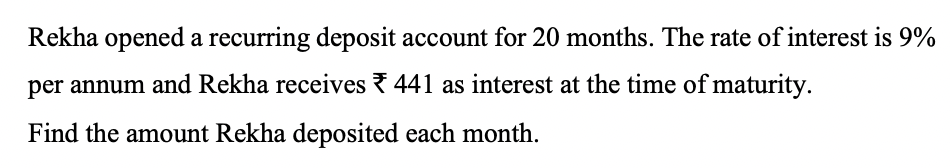
\includegraphics[width=\textwidth,frame]{question.png}

{\huge
Given,
Rekha opened a recurring deposit account for 20 months(n),
Rate of interest(r) is 9\% per annum,and Rekha receives \rupee 441 as interest at the time of maturity.
\\Let Amount deposited each month is \rupee x}
{\huge\\$$ From\;simple\;interest\;formula\;I=p\cdot\ t\cdot\frac{r}{100}
\\
\\
$$Total\;Interest(i) = x\cdot\frac{1}{12}\cdot\frac{9}{100} + x\cdot\frac{2}{12}\cdot\frac{9}{100} + x\cdot\frac{3}{12}\cdot\frac{9}{100} +
---- +x\cdot\frac{20}{12}\cdot\frac{9}{100}$$
\\
\\ $$Given\;Total\;Interest \; is \; 441 \; then$$
\\
\\$$441 = x\cdot\frac{9}{1200}(1+2+3+----+20)$$
\\
\\ $$x = \frac{441\cdot1200\cdot2}{9\cdot20\cdot21}$$
\\
\\$$ Finally\;we\;get \; x = 280 \;and\;c\;code\;output\;as\;follows
\\ }

{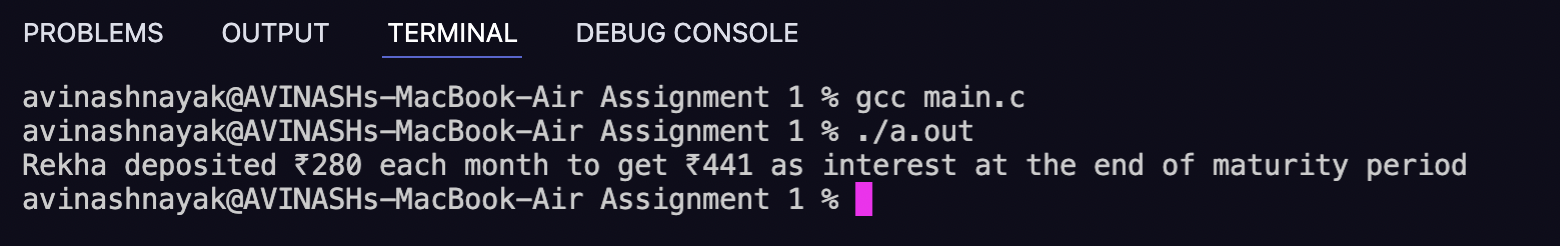
\includegraphics[width=\textwidth]{solution.png}}




\end{document}
